\documentclass[12pt]{article}
\usepackage{graphicx}
\usepackage{subcaption}
\usepackage[margin = 1in]{geometry}
\usepackage[parfill]{parskip}
\usepackage{float}
\usepackage{microtype}
\usepackage{newcent}
\usepackage{hyperref}
\hypersetup{
    colorlinks=true, 
    urlcolor=blue
}

\setcounter{section}{-1}
\linespread{1.5}
\setlength{\parskip}{12pt}

\title{On the Resources for Running a Splatoon Team}
\author{Tessaract Nonbinary Fuss }
\date{October 2024}

\begin{document}
\maketitle

\section{Disclaimer}
I've been captain of Nonbinary Fuss for about 2 years. These are the tools and resources I've accumulated over this time, and strategies that I find work for our roster. Your circumstances are likely to be different and some of this may either not apply to you or be helpful. This guide is also not on interpersonal relationships, moral, leadership, etc. This is the objective structure for how we function as a team and what I find helpful. 

I would strongly recommend \href{https://www.youtube.com/watch?v=Wtp-X-1W5rU&list=PLiBtcHtdkvJZk7OhLVf9o7qzIgXywZEID&pp=iAQB}{this video series made by Kale}. While there will be overlap, it does a great job at delving into how to form a team and especially handling the emotions of captaining. 



\section{Introduction}
As a 4 vs 4 team game, competing in Splatoon means you need at least 3 other people to play at any given point. For some players, they'd prefer to do pickups for tournaments and avoid a team structure. This is a valid way to approach the game, but not how I'd prefer to compete (nor what this guide is about). There is value in growing and improving with the same group of people, both from a community aspect but also the satisfaction of winning with friends. Doing well and succeeding is so much more satisfying when you celebrate as a team rather than an individual. 

Unfortunately those opting for being on teams run into the churn of disbanding. As I've played the game over the lifespan of Splatoon 3, our team has kept an internal list of every team we've directly interacted with that went on to disbanded. Though not exhaustive, it currently sits at nearly 60 teams. Obviously many teams will break up for interpersonal reasons or people losing interest in competing, but one of the issues is often difficulty organizing or improving. This means a lot of different things - not practicing very often, not doing tournaments, not keeping a schedule able to accommodate other people on the team well. Especially for people first beginning in the scene, captaining is a big responsibility and workload. Establishing a routine and clear communication on goals helps to remove some of the chaos that comes with running a team.



\section{Scheduling Structure}
\subsection{Availability}
Approaching a schedule week by week is the most flexible both for your team and with the community. Family events, work schedules, homework, vacations, and more all tend to not be known a month or more in advance. Building a schedule with this time frame in mind lets people fit their lives around a comp schedule with some advance notice, but not the pressure of knowing how free you'll be 3 Tuesdays from now. This also fits into the volatility of some tournaments, as they can move around or be canceled too. 

Some teams take the approach of having set days for certain activities - practice on specific weekdays and doing specific weekly tournaments that are always on the same day too. This is the simplest approach but also allows for very little flexibility. We prefer to build the schedule week by week, generally sticking to trends for when scrims/tournaments will tend to happen but allowing it to float. We don't have set "practice days", but for example scrims tend to happen earlier in the week with VOD reviews later on.

Tools like Doodle and LettuceMeet exist, but they don't serve this role especially well from experience. We've found great success in Rallly, a free and open source tool to create a poll each week. Importantly this isn't the final schedule - instead a quick check for how free people are on each given day. Someone can be available every single day of the week, but they might not have the stamina or interest to do activities for all 7 days. Rallly is intentionally simple and doesn't specify events on each day. Teammates don't need an account to fill it out, can mark yes/no/maybe, and can edit their answers after submitting. This gives a baseline for people's availability to make the schedule.

After knowing which days have 4 people free, you can start to create Discord server events corresponding to team activity. These events have the advantage of being baked right into your server and easily accessible by teammates. Each event requires you to mark it as interested, and this is the confirmation that someone is free to do that event at that day/time. Your teammates have to deliberately confirm to each event, and will get notifications after doing so from your Discord server. 
\begin{figure}
    \centering
    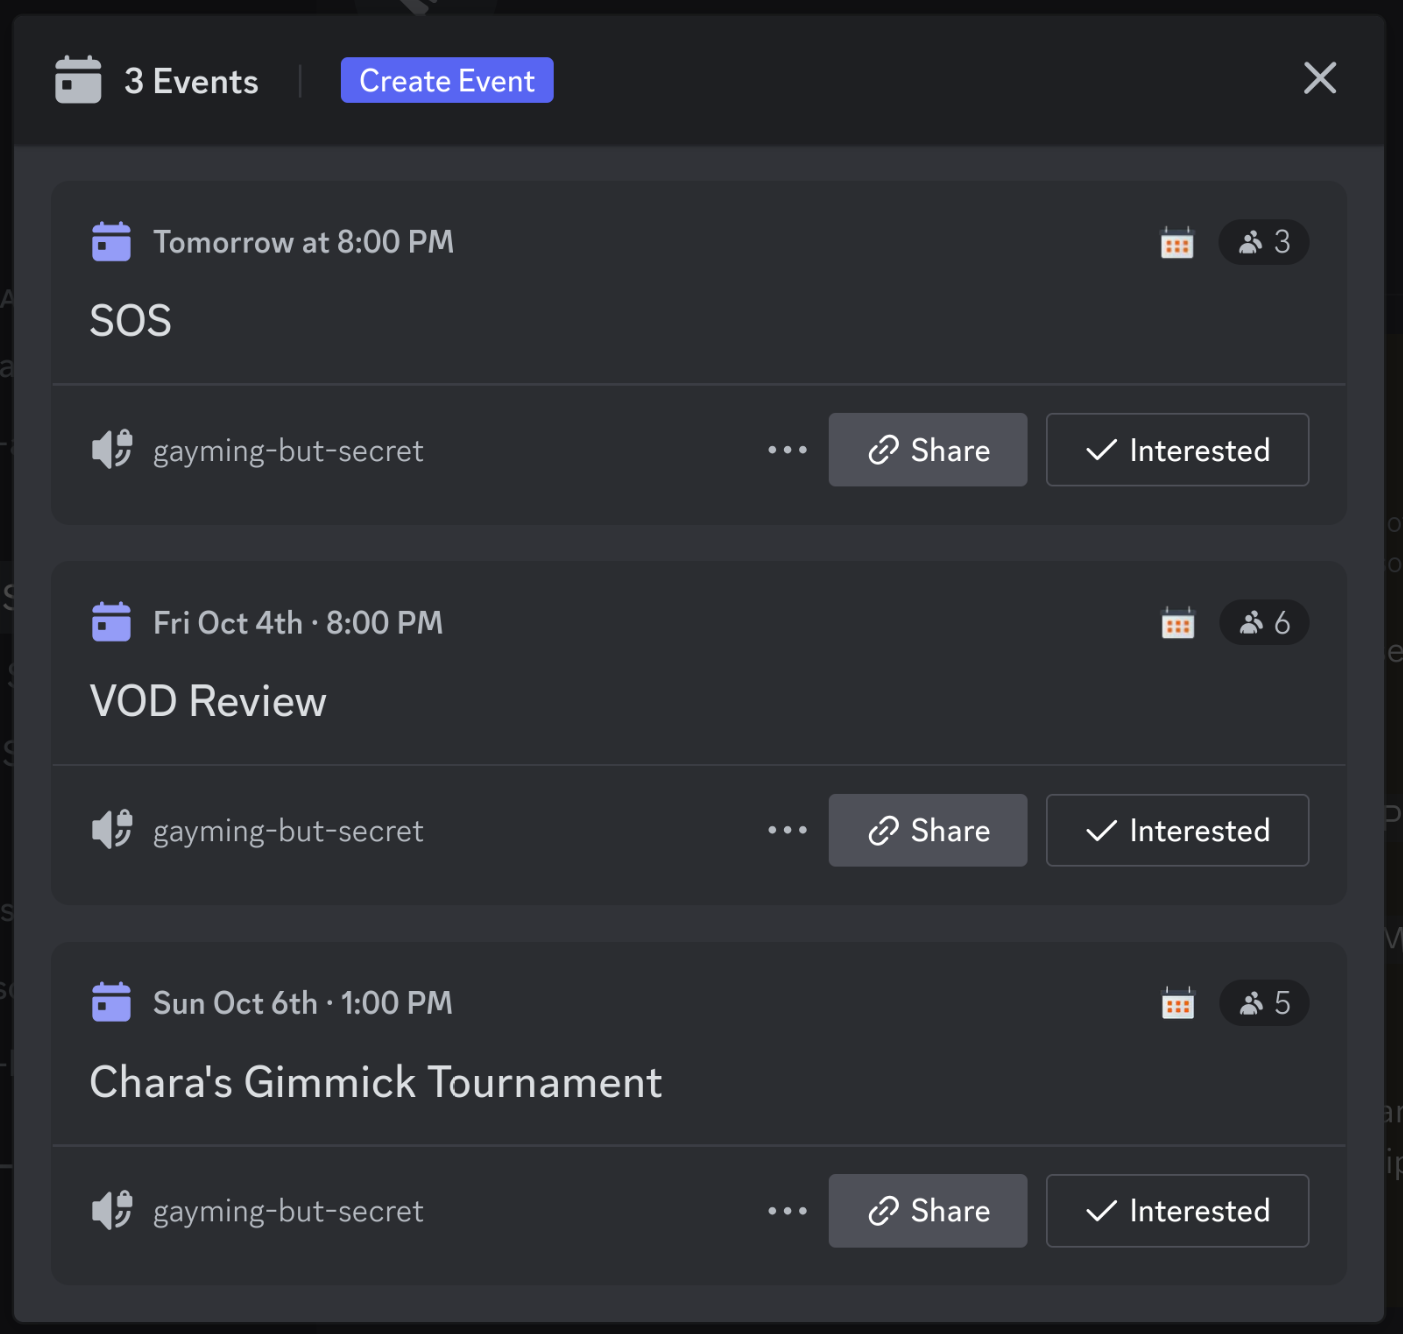
\includegraphics[width=0.6\linewidth]{discord_events.png}
\caption{Events in the Nonbinary Fuss Discord server created by ChronicleBot}
\end{figure}

\subsection{Goals}
Part of improving is not just fundamentals like coordination or mechanics, but also deliberately focusing on and addressing weaknesses. Practice during a scrim or solo queue is much more effective when you have some smaller thing to improve, rather than trying to get better at everything at once. These goals don't need to be big, examples like opening your map more often or calling out when using a special are things you can evaluate at the end of the week to see if you've improved. Loftier ambitions like winning a tournament or reaching mid-level/high-level aren't something achievable in a short time span. Of course you can still have these goals and work towards them, but you get there by improving on the smaller things first. If you still need improvement on a week's goal, you can roll it over into the next week to keep chipping away at it.
\begin{figure}
    \centering
    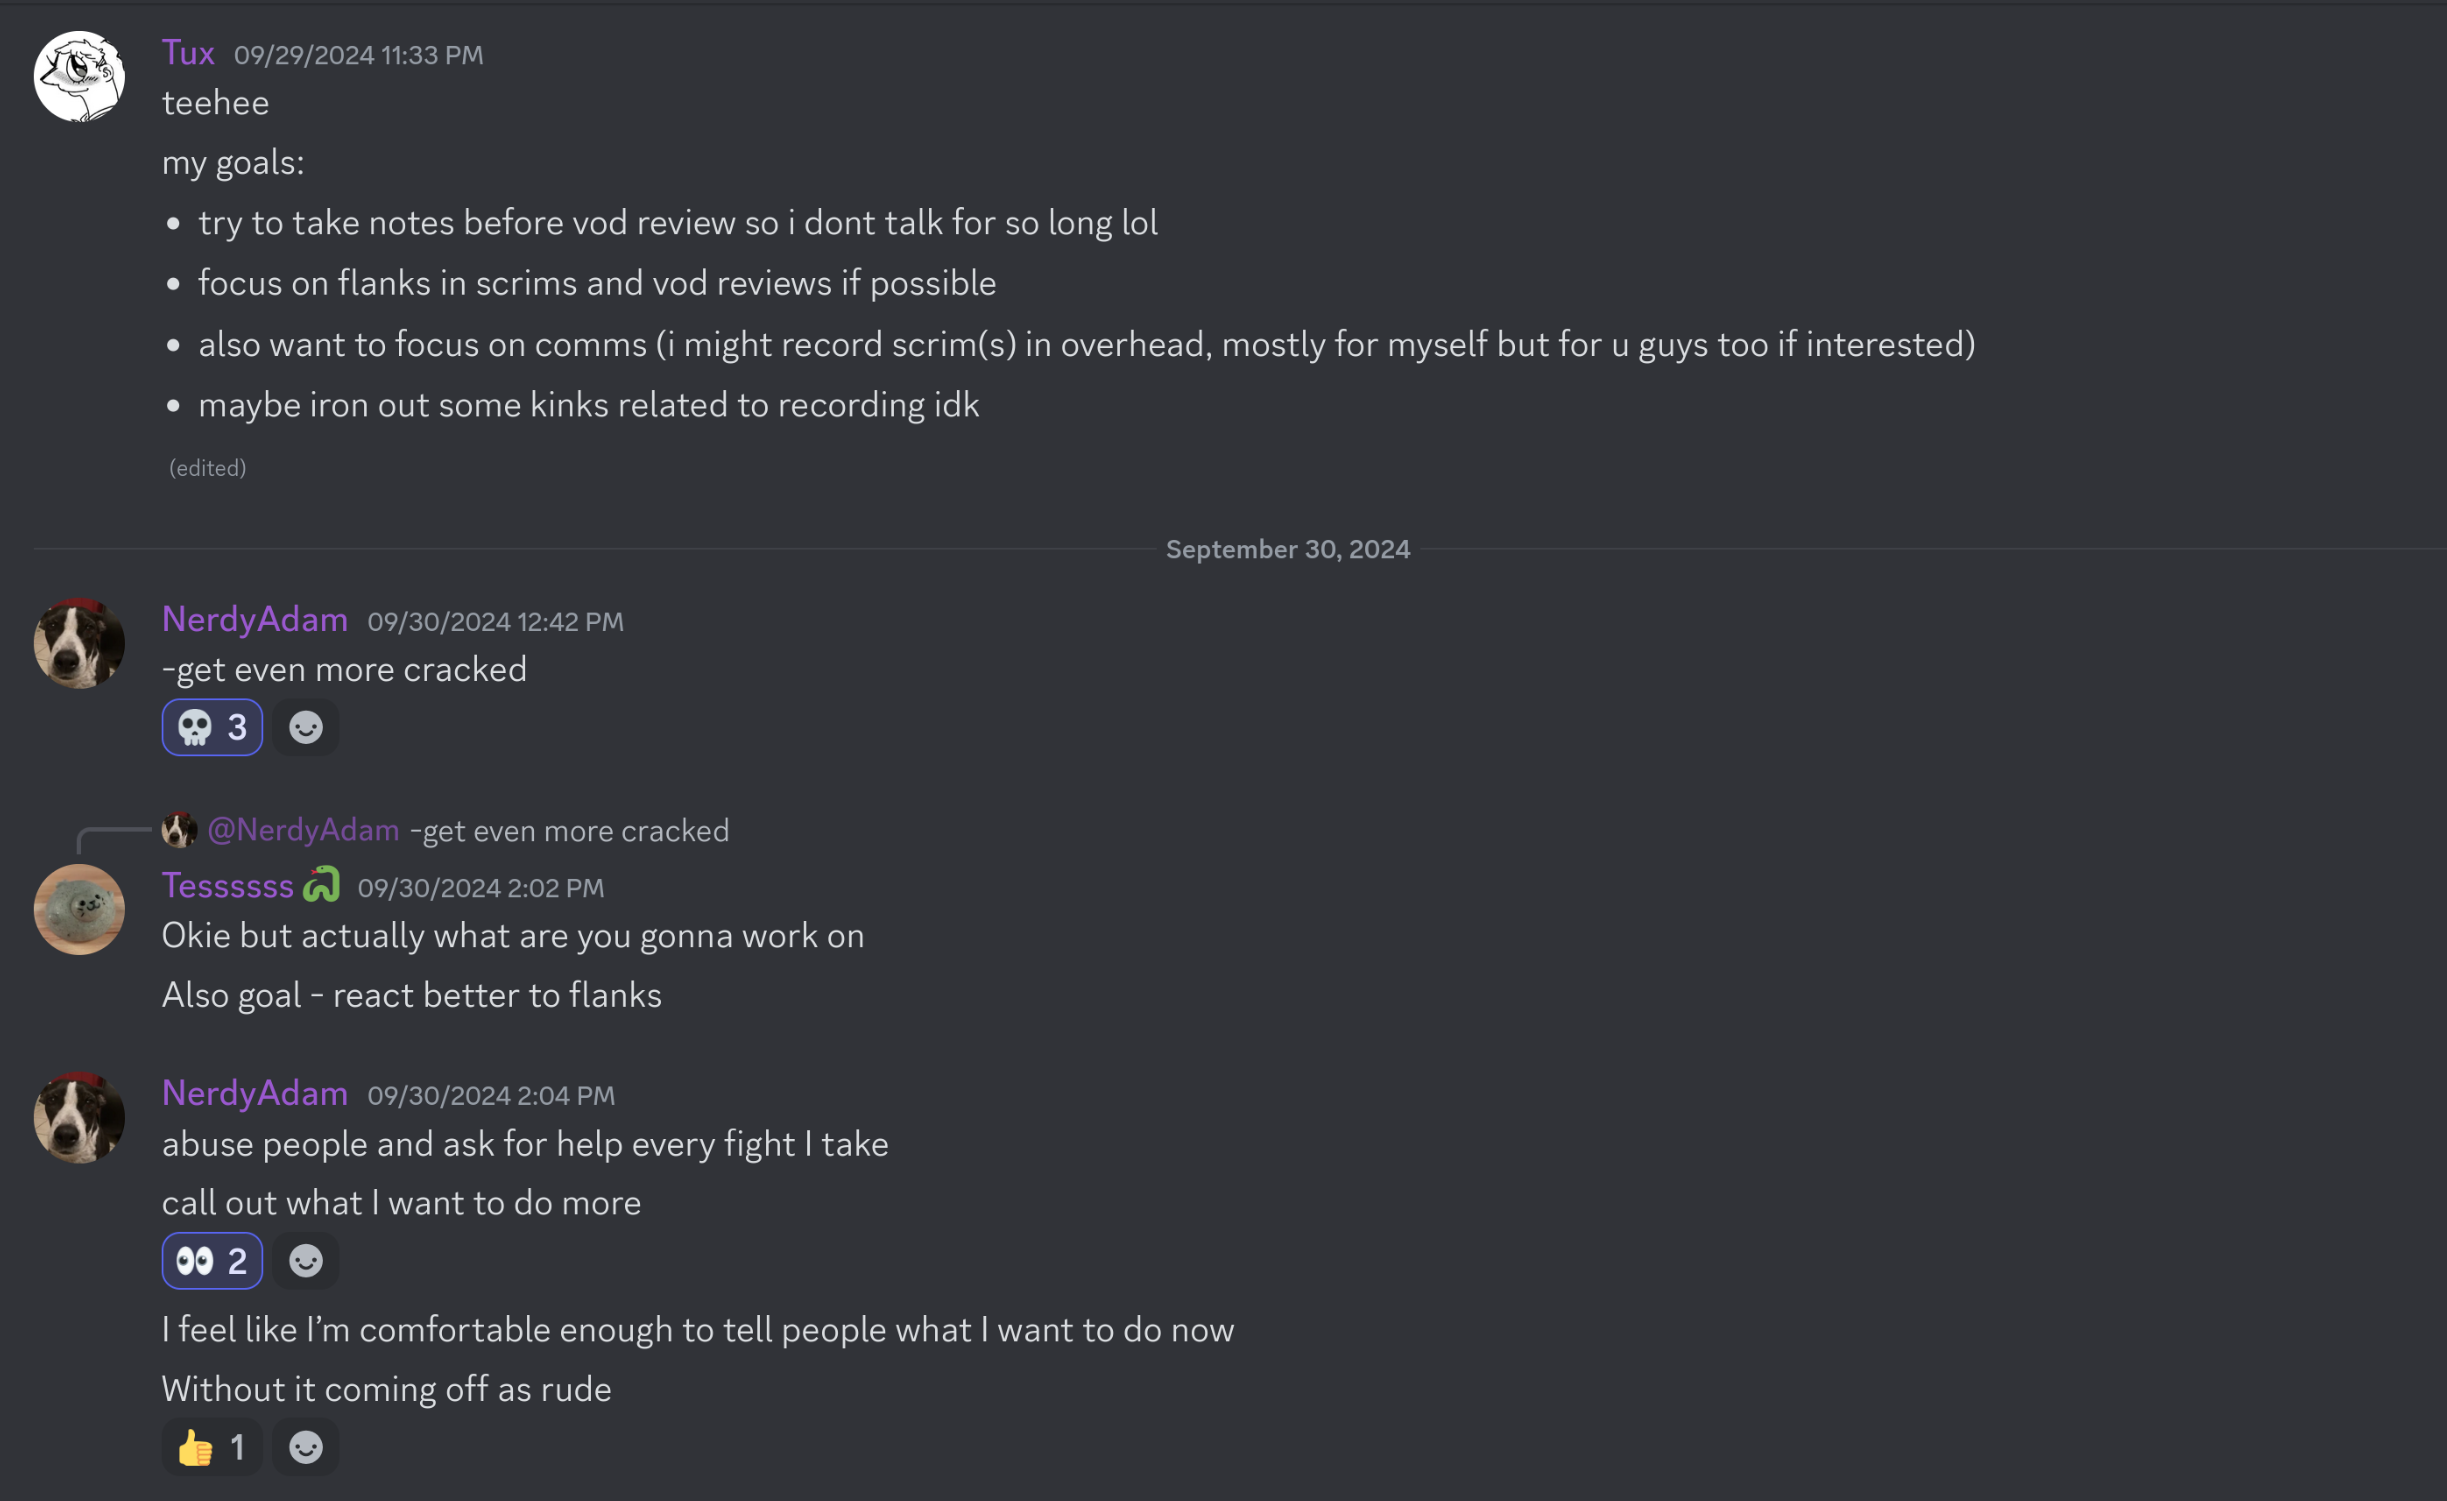
\includegraphics[width=.95\linewidth]{discord_goals.png}
\caption{Example goals made by members of Nonbinary Fuss}
\end{figure}

\section{Infrastructure}
\subsection{Discord}
A dedicated server for your team is a great place to keep communication between members and interact with the community. How you structure your server and who you invite is up to you, but you'll want a separate team category with private channels just for you and your teammates. Beyond a private team chat and VC, you should have a channel dedicated to planning. This allows for any logistics to stay in an easily accessible place without being buried in other discussions or channels. We make a thread for each week to further organize things and post what possible events we could do. 
\begin{figure}[H]
\centering
    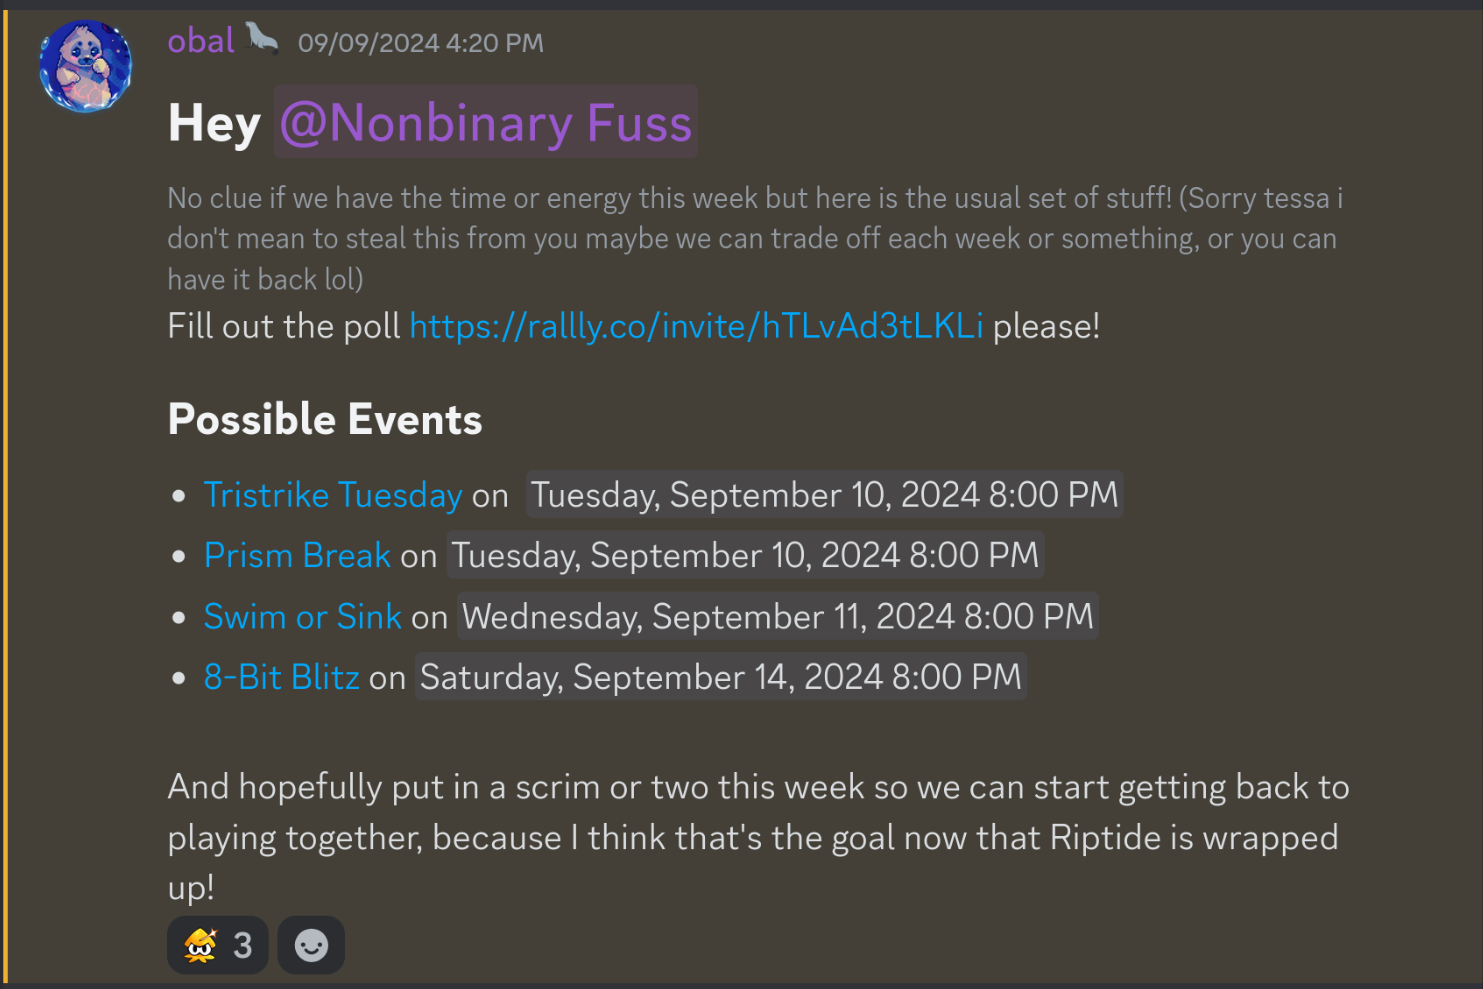
\includegraphics[width=.95\linewidth]{discord_planning.png}
\caption{An example weekly post from the Nonbinary Fuss Discord server}
\end{figure}

In particular, we leverage ChronicleBot to manage scheduling. After we know our team's rough availability via Rallly, I'll create events in Google Calendar for specific plans like a scrim or tournament. ChronicleBot will sync this to our Discord server's events, and allow people to click interested to RSVP. This has the added benefit of allowing anyone to pull from the Google Calendar onto their own personal Calendar to better keep track of events. \href{https://chroniclebot.com/docs/notifier/discord-event-sync#voice-channel-events}{By setting the location accordingly}, you can even have the event go to your desired voice chat.
\begin{figure}
\centering
\begin{subfigure}{.58\textwidth}
    \centering
    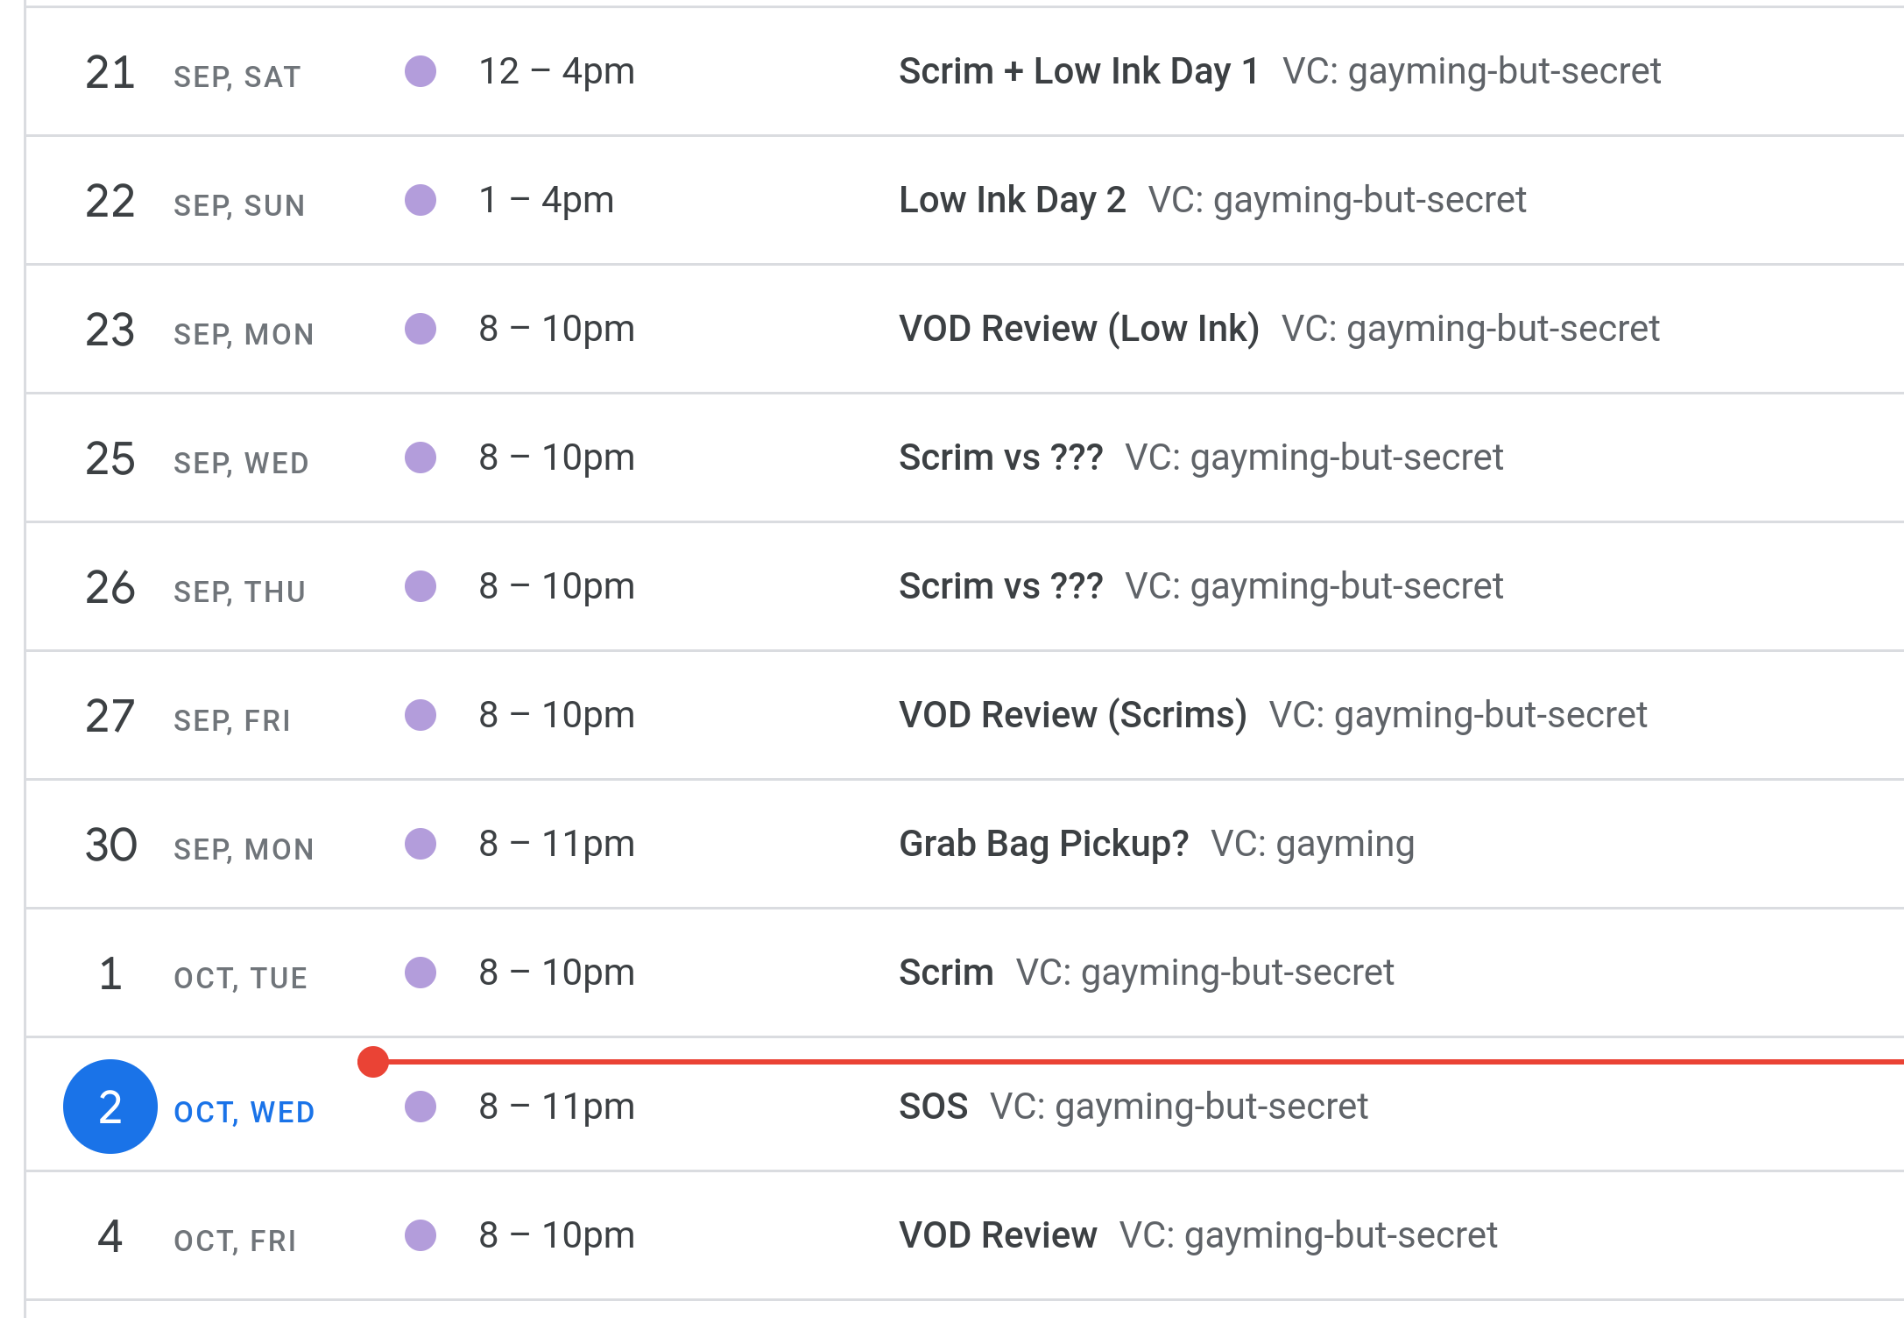
\includegraphics[width=.95\linewidth]{google_calendar.png}
    \caption{Team events entered into Google Calendar.}
\end{subfigure}%
\begin{subfigure}{.42\textwidth}
    \centering
    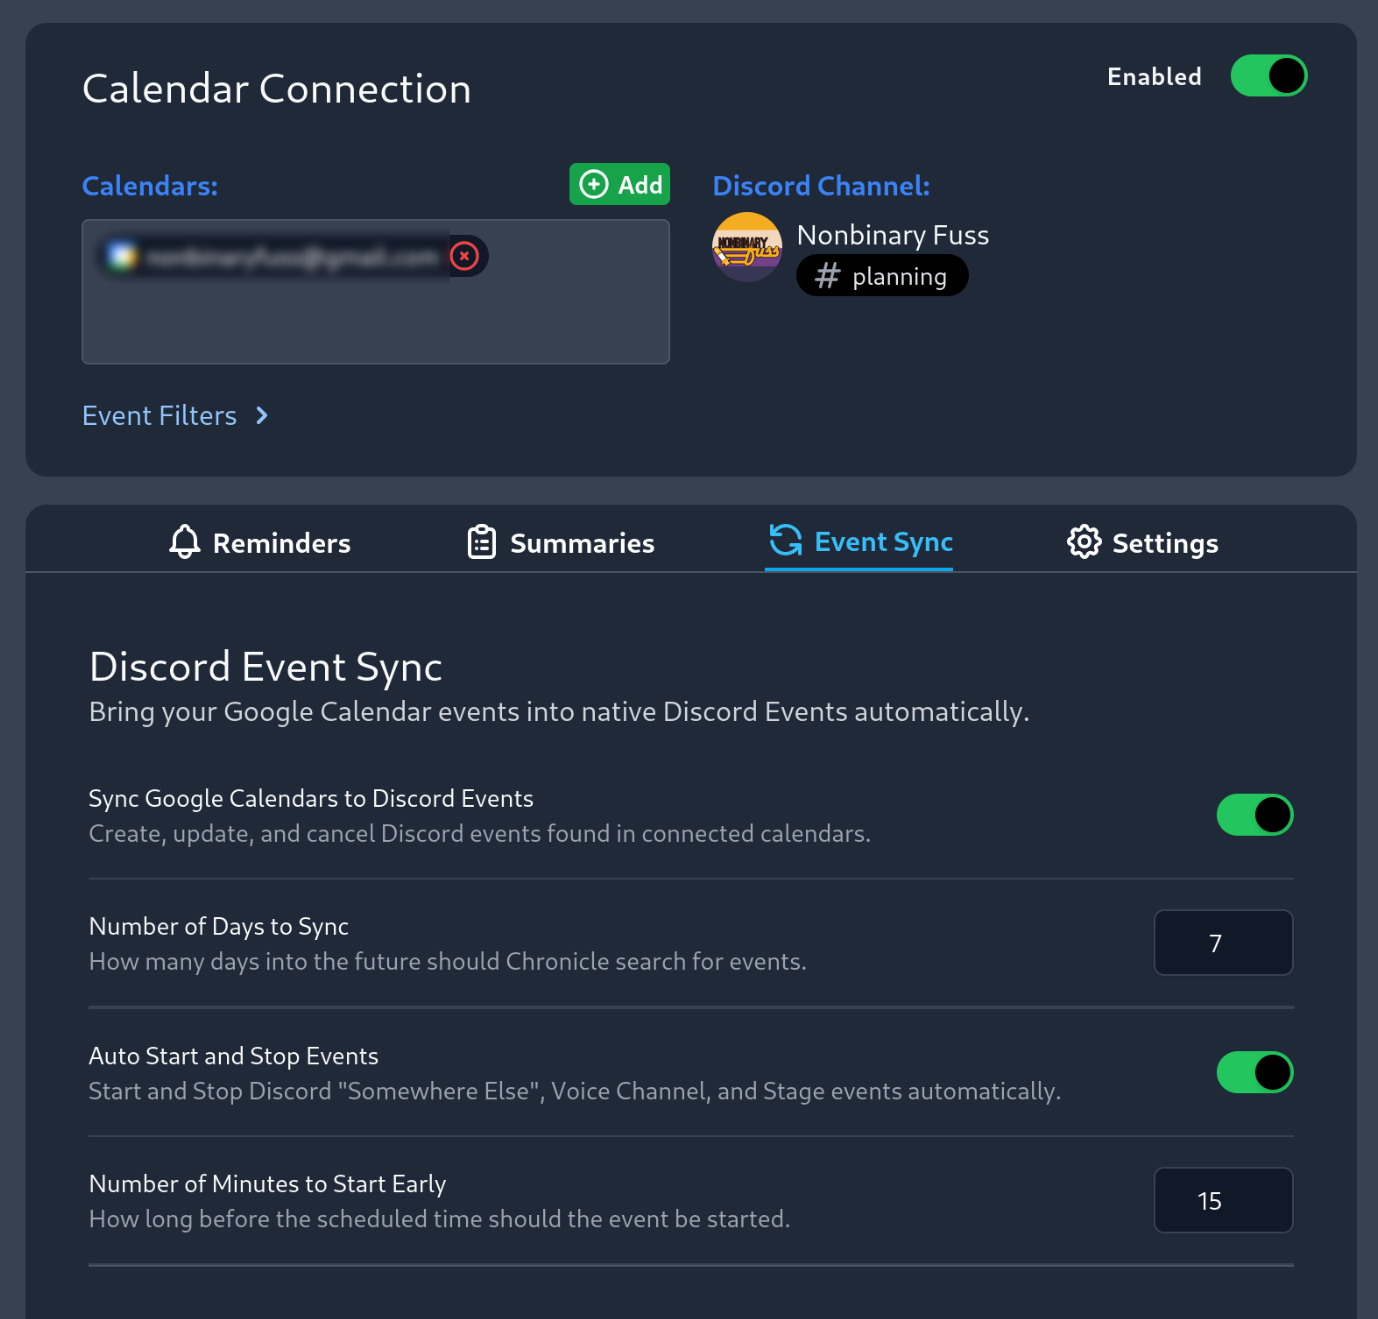
\includegraphics[width=.95\linewidth]{chronicle_bot.png}
    \caption{ChronicleBot configuration}
\end{subfigure}
\caption{Setup to sync Google Calendar entries into Discord}
\end{figure}

\subsection{Rallly}
My preferred way to gauge availability for the week is \href{https://rallly.co}{Rallly}. An account isn't required to respond, and any dates/times are automatically converted into your timezone. The interface works well on small screens, meaning your teammates can easily answer on their phones. Typically I ask for availability at 8-10 pm EST everyday that week (as we play around then and tournaments tend to start at 8 pm EST), and 1-4 pm EST on Saturday/Sunday if there are any weekend tournaments. For LUTI scheduling, I'll get more granular on each day just to narrow down the exact time for a set and avoid confusion.
\begin{figure}
    \centering
    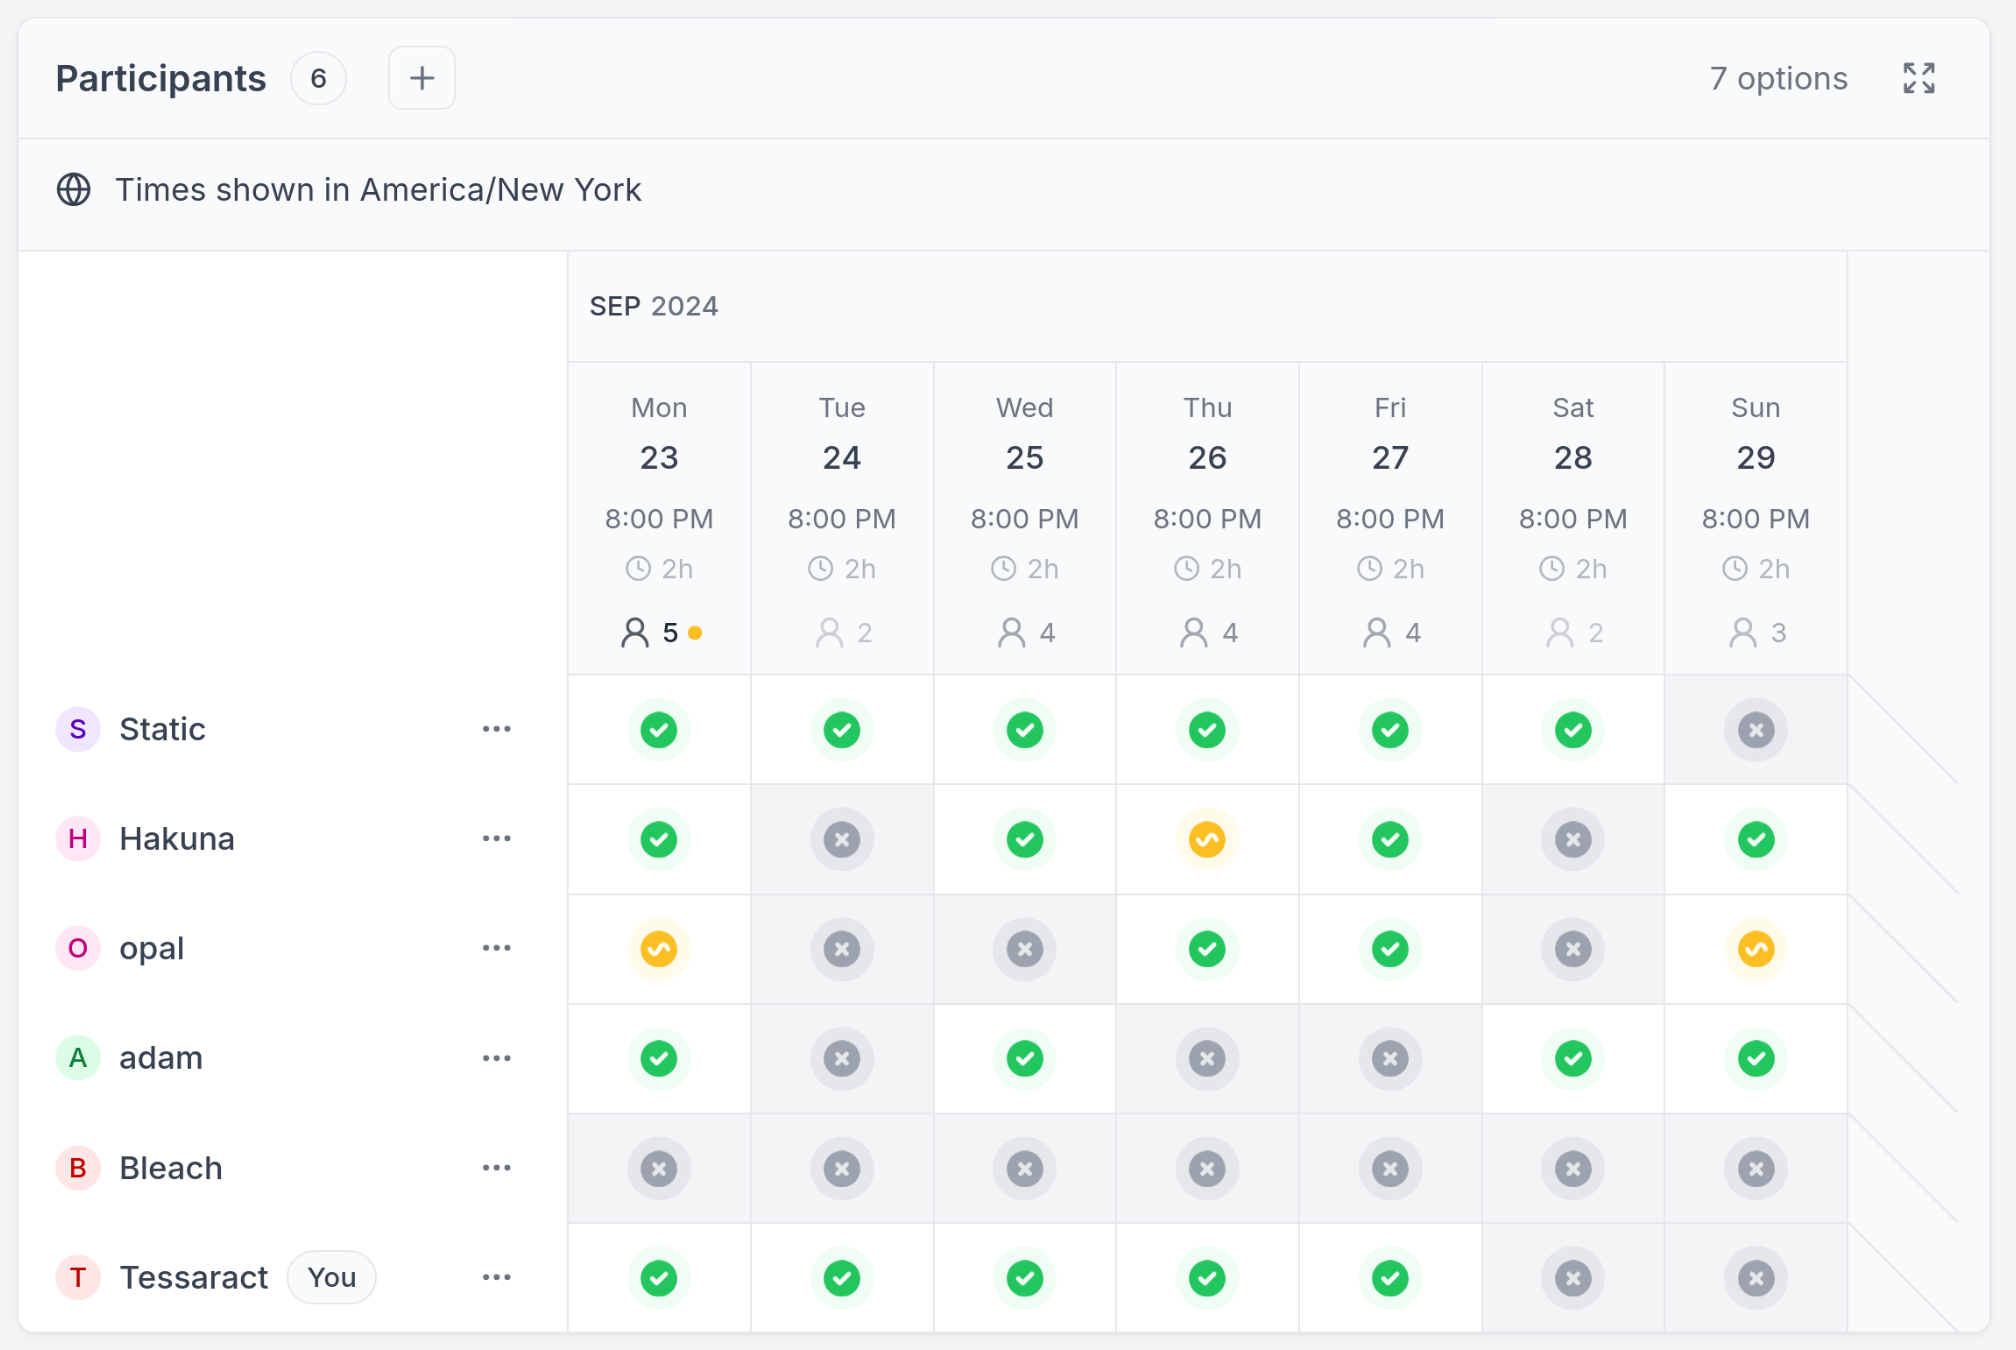
\includegraphics[width=0.8\linewidth]{rallly.png}
\caption{Rallly weekly availability polling.}
\end{figure}

\subsection{Google}
Having a team Google account is helpful in providing a number of services - Gmail, Google Calendar, Sheets, etc. A team email via Gmail will allow you to sign up for accounts on sites like Bluesky, Carrd, Notion, etc. and not tie the associated email to any one team member. 

Google Sheets is how we organize results, with multiple columns corresponding to results based on the skill cap (open/div 5/div 7). Every single tournament placement is recorded here, alongside some pickups containing 1-2 team members. Although we didn't structure our spreadsheet this way, you could track sets or who participated in each tournament result. Ultimately how much or little you want to record is based on personal preference. 
\begin{figure}
    \centering
    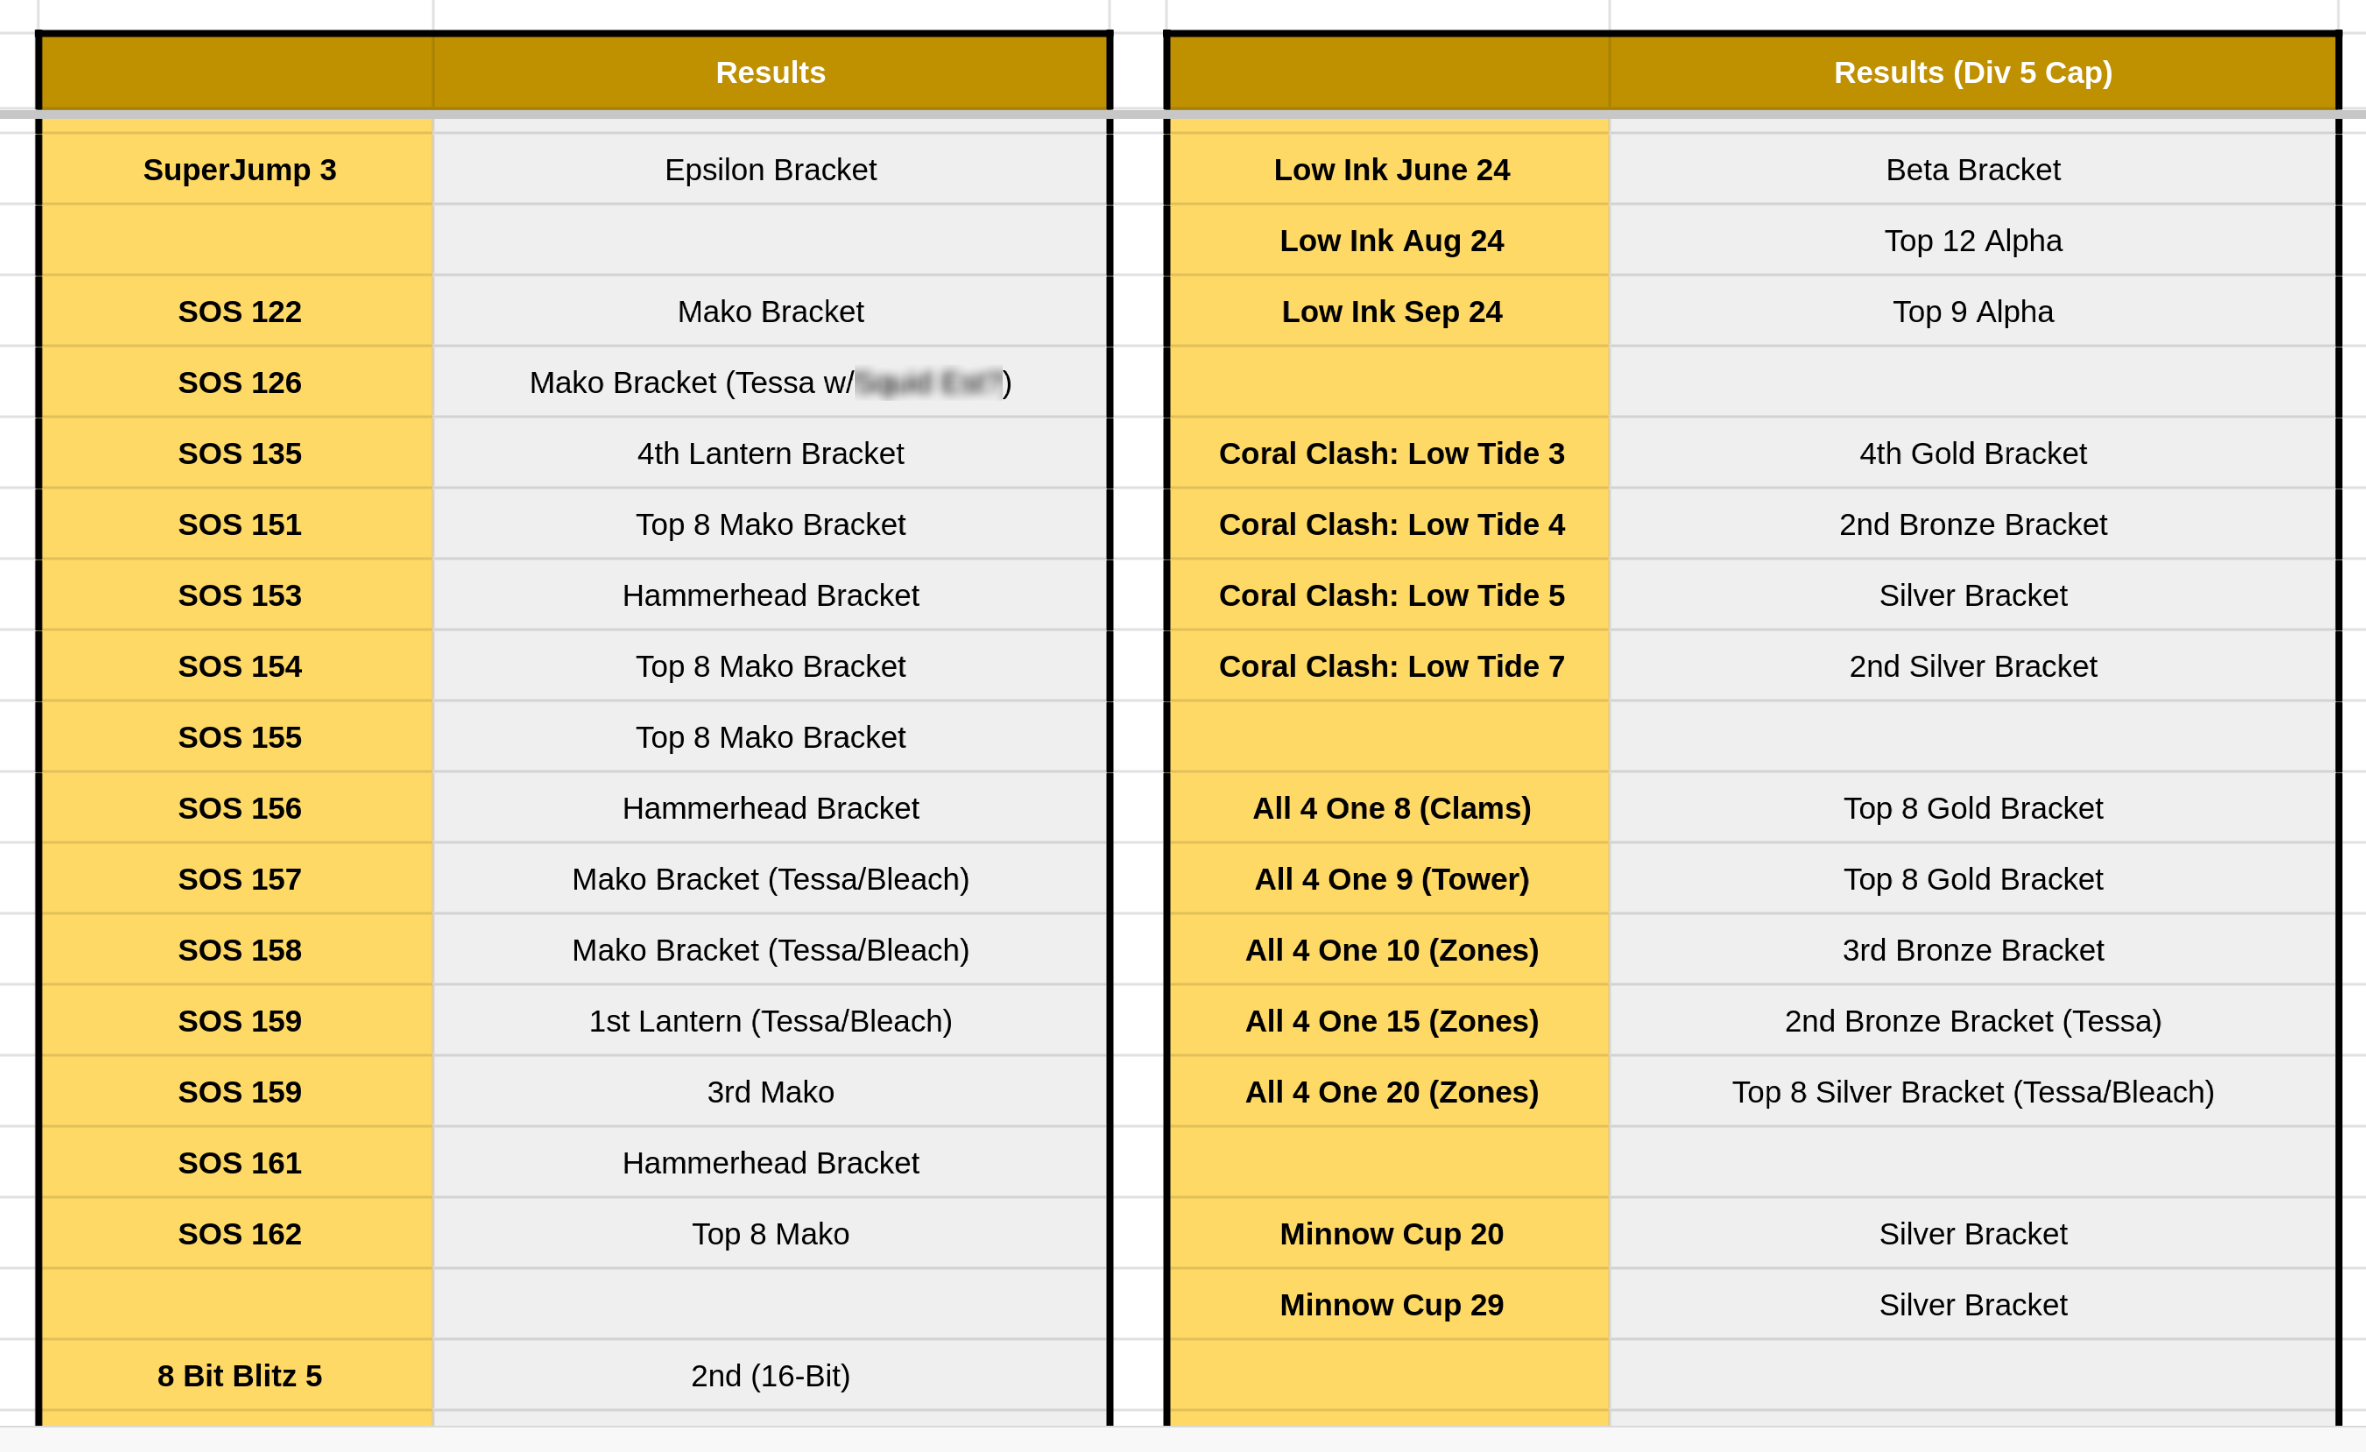
\includegraphics[width=1\linewidth]{google_sheets.png}
\caption{Some results from Nonbinary Fuss in Google Sheets}
\end{figure}

A team Youtube account (using said Google account) is also where we store VOD review recordings. Any VOD review is always recorded (and uploaded unlisted) so that anyone who misses it can watch it back later on their own time. You can choose to also post recordings of scrims/tournaments either privately or publically, though we tend to have our Youtube channel fairly dormant otherwise.

\subsection{Bluesky}
A team \href{https://bsky.app}{Bluesky} is useful in building up a presence outside of your Discord server to show off achievements and build clout. Taking a team photo and posting about your tournament experience is a fun bonding exercise and allows you to celebrate your achievement with the entire community. In some ways this is similar to almost having "corporate branding", but you can also use it to highlight other teammate's posts, make memes, and in general make your team more recognizable. Tagging posts with \href{https://bsky.app/profile/kibryhouse.bsky.social/feed/comp-splatoon}{\#compsplatoon} makes them more visible to others via the Competitive Splatoon feed.

\subsection{Broadcast Box}
Discord streaming and screensharing is middling quality at best, with poor bitrates and network issues even for people with fast internet. We've recently discovered \href{https://github.com/glimesh/broadcast-box}{Broadcast Box} as an alternative, a tool able to stream from OBS with low latency and high quality. After setting a stream key and pointing to the server in OBS, you can easily stream to anyone using the site. This has been useful for VOD reviewing, with the latency of Twitch or Youtube making active discussion about what's happening almost impossible. Note that our experience has been that it only works well on Firefox (and you should switch to Firefox regardless!).
\begin{figure}[H]
    \centering
    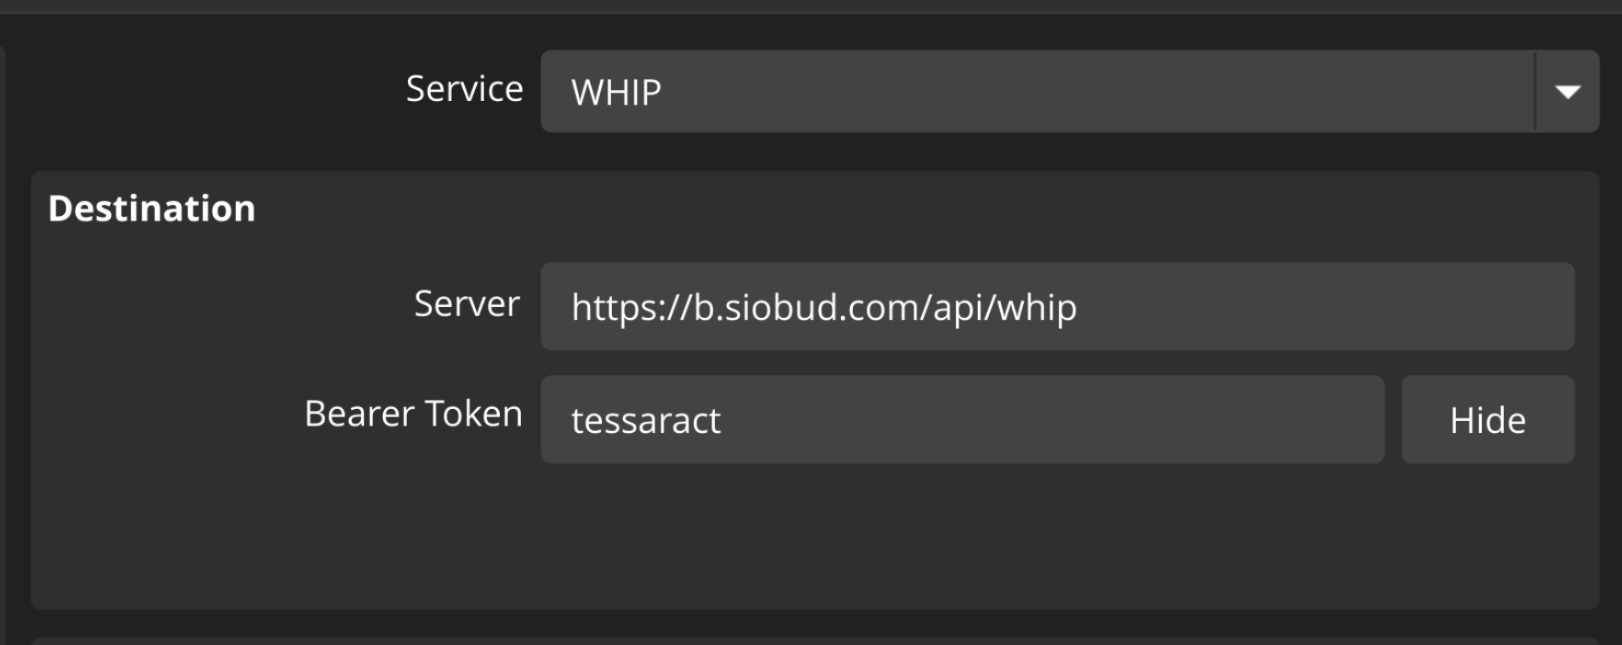
\includegraphics[width=0.7\linewidth]{broadcastbox.png}
\caption{Configuration in OBS to stream to \href{https://b.siobud.com/tessaract}{https://b.siobud.com/tessaract}}
\end{figure}

\subsection{Simplenote}
For some information, it's helpful to have in a collaborative list but not as clunky as a full Google Doc/Sheet. \href{https://simplenote.com}{Simplenote} is just that, simple text documents you can publish and link to without the app. It also has markdown support for more control over formatting. Depending on preferences, tables in a document could even be used in place of a full Google Sheet.



\section{Weekly Events}
Joining certain community servers is almost essential in being able to find scrims. Note that these links could be expired, so be sure to check their Bluesky pages if necessary. 
\begin{itemize}
  \item \href{https://discord.com/invite/sendou}{Sendou.ink}
  \item \href{https://discord.gg/F7RaNUR}{Inkling Performance Labs}
  \item \href{https://discord.com/invite/0dZpaQB1mwcd2MCs}{LUTI}
\end{itemize}

\subsection{Scrims}
Scrim partners are the most reliable way to schedule scrims. If you're familiar with 3-5 teams around your skill level, you can reach out to them on days your team tends to scrim. My strategy for finding them is to pay attention to any close sets in a tournament, and reach out to that team's captain afterwords. In the scenario you can't find their captain, check their team's Sendou page or Bluesky account If they're interested in scrimming, you now have a contact to reach out to when planning your week. We tend to cycle scrim partners as we grow in skill, both to keep up the challenge and to face different team styles/compositions.

If you don't have someone to reach out to, some larger tournament Discord servers like IPL will have channels that let you ping for other teams. You'll want to include a time and estimated skill level, but it can also be helpful to list any restrictions like the scrim being short or needing to ban splattercolor screen. Another option is Scrimboards, a tool embedded in some servers like LUTI. You can create a post looking for a scrim, and it'll show up on any other server using Scrimboards too. You can also browse other team's posts and accept an available scrim, prompting you to message their captain for details. 

If you still can't find a scrim by the time slot you have scheduled, SendouQ is another option. This can be hit or miss depending on activity levels, but 1-2 sets can be a good substitute for a scrim.

\subsection{Tournaments}
Most tournaments are now on sendou.ink, and even those that aren't tend to be listed on the site's \href{https://sendou.ink/calendar}{calendar}. Many tournaments tend to happen on the same days/times at regular intervals, so you can plan around something like Swim or Sink always being on Wednesday at 8 pm EST. Some tournaments are labeled as skill capped, meaning they can cater to low/mid-level teams specifically. In contrast, others are open registration and allow any team to join. Most tournaments have multiple brackets, meaning that you'll get a chance to fight teams closer in skill level once the groups stage is done.
\begin{figure}
    \centering
    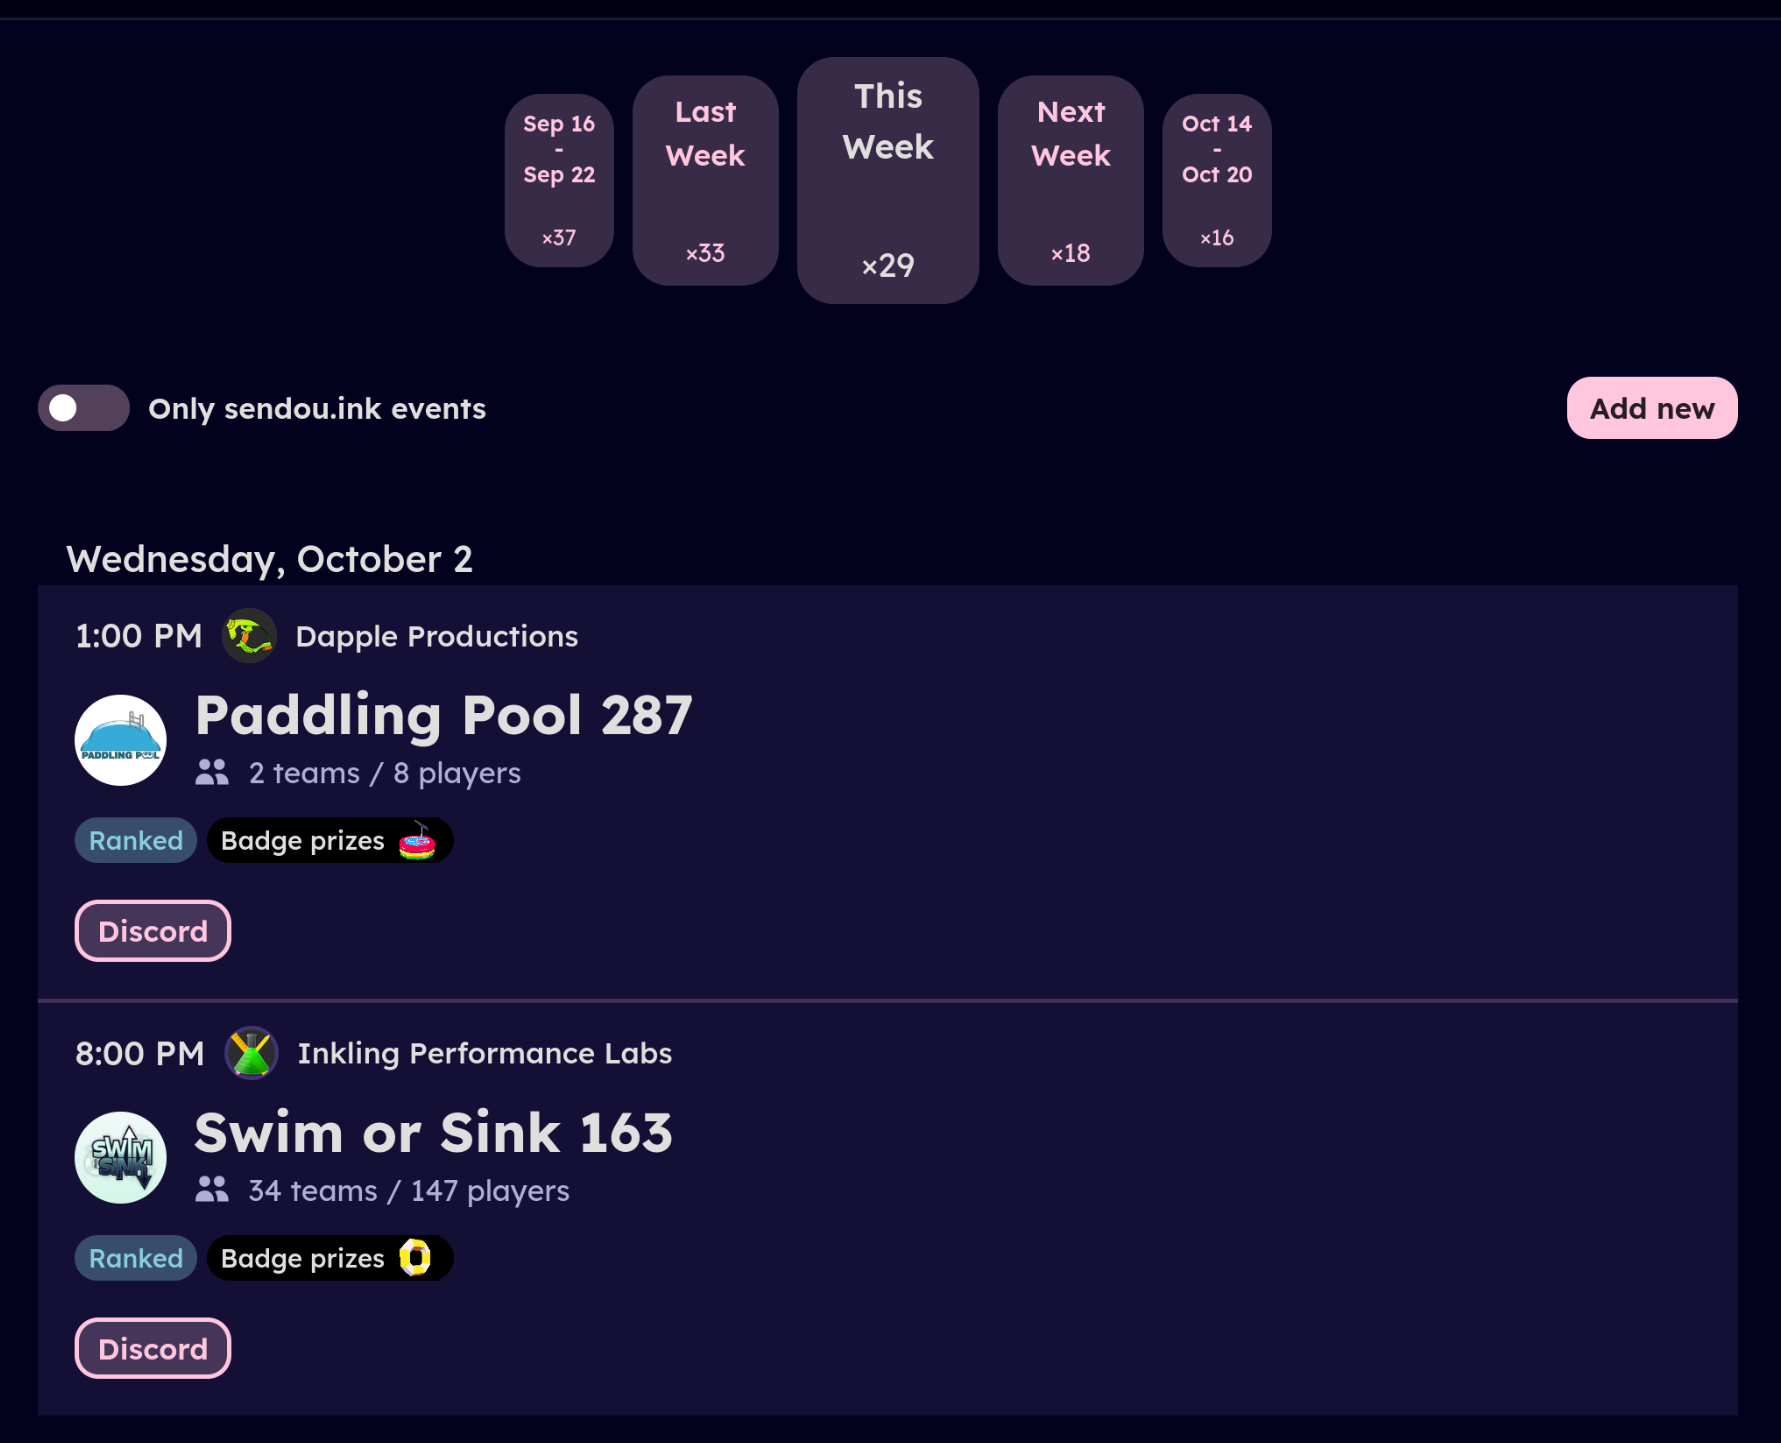
\includegraphics[width=0.8\linewidth]{sendou_calendar.png}
\caption{Tournaments on the Sendou.ink calendar page}
\end{figure}

\subsection{VOD Reviews}
Towards the end of each week, we'll do a review of 2-4 games from scrims/tournaments that we either made notable mistakes in or need improvement on. After watching through a game from an overhead perspective, we'll go back to moments that we noticed good plays or mistakes. This typically prompts good discussion about individual intentions in the moment, and collaboration on what we'd do differently going forward. The critical thinking to critique a mistake and notice a good play will improve your decision making in the future, which is why VOD reviewing is so vital to improvement.



\section{Division of Labor}
As mentioned earlier, managing every aspect of a team is difficult and time consuming. Part of being captain is also delegating work to other teammates, both for your own sanity and to help them improve on skills like communication and organization. Splitting the workload also helps ensure the team can run smoothly in circumstances in which the captain is unavailable or busy. Often it makes most sense for the captain to orchestrate scheduling/availability each week.

\subsection{Scrim Manager}
Each week, this person is responsible for finding scrims for days the team plans to practice. They are in charge of reaching out to other teams and coordinating on a time/date for a scrim. Maintaining a list of scrim partners or server to ping other teams helps streamline the process, especially if the person in charge is swapping each week. Typically they also are the ones to communicate with the other team during the scrim, helping to set up the maplist, subbing players out if they're hosting the room, and asking for replays/breaks.
\subsection{Replay Leader}
This person is in charge of leading replay reviews each week. They'll pick out 2-4 games from a scrim or tournament each week and stream the VOD review. They should generally be prompting discussion and pointing out areas they noticed in each game that either need improvement or were well executed. The VOD review should ideally also be recorded and uploaded to a team Youtube channel (unlisted) both to reference in the future and share with teammates who weren't able to attend that day.
\subsection{Organizer}
Less of a role to be swapped but more a permanent job, their job is to maintain a spreadsheet of team results and lead goals discussions each week. Generally this is best done via a new thread for each week in a dedicated channel, and teammates should be reminded to write down a goal if they don't do so early in the week. 



\section{Conclusion}
Although captaining a team can be daunting, breaking the weekly tasks down into a routine can help to reduce stress and distribute the workload to teammates. By using these organizing tools, it has helped me immensely in clarity of information and transparency in scheduling to my teammates. Especially operating as a team of 6 plus a coach, we're allowed the flexibility to take weeks/days off without impacting the team as a whole and to do so clearly. Information stays organized in our server, events are plainly visible, expectations are set before the week begins. As I've accumulated these tools over two years of captaining, I hope they can help others in more regularly competing and avoiding internal conflict. 

With the discourse and discussion around a lack of teams, the hope is that this guide in the long term enables existing teams to trickle upwards as they improve. Though pickup culture at higher levels of play has reasons beyond team organization issues, more teams reaching mid and high level and staying together can slowly lead to a cultural shift.

\end{document}